\renewcommand\labelitemi{-}
\renewcommand\labelitemii{$\circ$}
\renewcommand {\thesection}{\arabic{section}}

\chapter*{Introduction générale}
\addcontentsline{toc}{chapter}{Introduction générale}
Selon le centre national de prévention et de sécurité routière algérien : 
plus de 3.049 personnes avaient trouvé la mort et 29.095 personnes avaient été blessées
 dans 21.109 accidents enregistrés au niveau national lors des onze premiers mois de l'année 2019  \cite{nassimaAccidentsRouteAlger}.
 \begin{figure}[h!]
  \center
  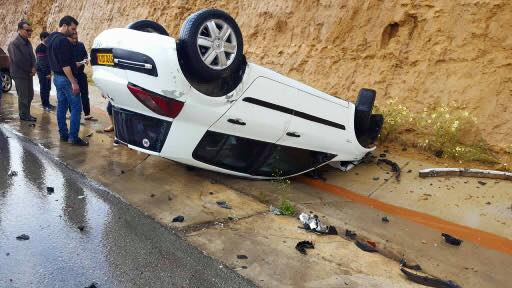
\includegraphics[width=0.75\textwidth]{Images/chapter1/accident.jpg}
 \caption{Accident de route}
 \label{fig:Accident}
  \end{figure}
  Dans un scénario réel, la règle dit que plus la surface de la route est confrontée
   à des changements de climat (entre le froid et le chaud) et avec un manque de soins, 
  plus elle subit des dégâts et affecte ensuite la vie des gens.\newline
  La surveillance de la surface des routes est un problème difficile dans le domaine des 
  infrastructures de transport routier dans le monde entier. Une zone en mauvais état peut 
  endommager les véhicules, les conducteurs et même provoquer un accident. 
  Ils sont également à l'origine de poursuites et de dommages-intérêts coûteux, par exemple, 
  en 2005, l'État du Michigan avait déposé plus de 7,500 réclamations pour dommages liés 
  aux nids-de-poule \footnote{http://www.detnews.com/2005/specialreport/0510/18/A01-350197.htm}, et les 
  compagnies d'assurance recevaient plus de 500,000 réclamations pour nids-de-poule chaque 
  année\footnote{http://www.wktv.com/special/6733696.html}.\newline
  Les municipalités du monde entier dépensent des millions de dollars pour entretenir et réparer leurs routes\footnote{http://boston.bizjournals.com/boston/othercities/denver/stories/2007/04/02/story1.html?b=1175486400\%5E1438887}.
  Malgré cet investissement, peu de gens sont satisfaits de la qualité de la route où ils vivent ou travaillent, car c'est  toujours trop tard!! 

  \section{Problématique}
  De ce qui précède,l’entretien et la maintenance de la qualité de l'infrastructure routière est d'une importance vitale pour la société.\newline
  En Algérie particulièrement, ce domaine est presque négligé, les routes endommagées sont plus que les routes sûres.\newline 
  L’entretien de la route en Algérie  passe par plusieurs phases : 
      \begin{itemize}
          \item Détection des dégradations.
          \item Localisation des dégradations : les agents du service de contrôle de la route utilisent les points kilométriques 'PK'. pour localiser les dégradations.
          \item L’entretient de la route se fait soit par la direction des travaux publics 'DTP' ou une entreprise désignée par le Ministère des travaux public 'MTP'. 
      \end{itemize}
  La détection des dégradations jusqu’à présent se fait par constatation visuelle par des agents d’entretien de la DTP, cette étape est fastidieuse et longue nécessitant un savoir-faire particulier et une expérience dans le domaine. Par cela; les dégradations (nids-de-poule/bosses) prend beaucoup de temps pour être réparées et par conséquent elles causeront plus de dégâts.

  \section{Anomalies dans une route}
Dans nos recherches lors de l'étude du domaine problématique, nous observons que les anomalies
 les plus courantes sont les nids-de-poule (potholes) et les bosses(bumps).
  Ces deux catégories peuvent classer la plupart des anomalies trouvées dans notre vie quotidienne. Ainsi, nous avons:

  \subsection{les nids-de-poule}

Les nids-de-poule sont principalement causés par une mauvaise qualité de la chaussée ou des problèmes sous la surface.
\begin{figure}[h!]
  \center
  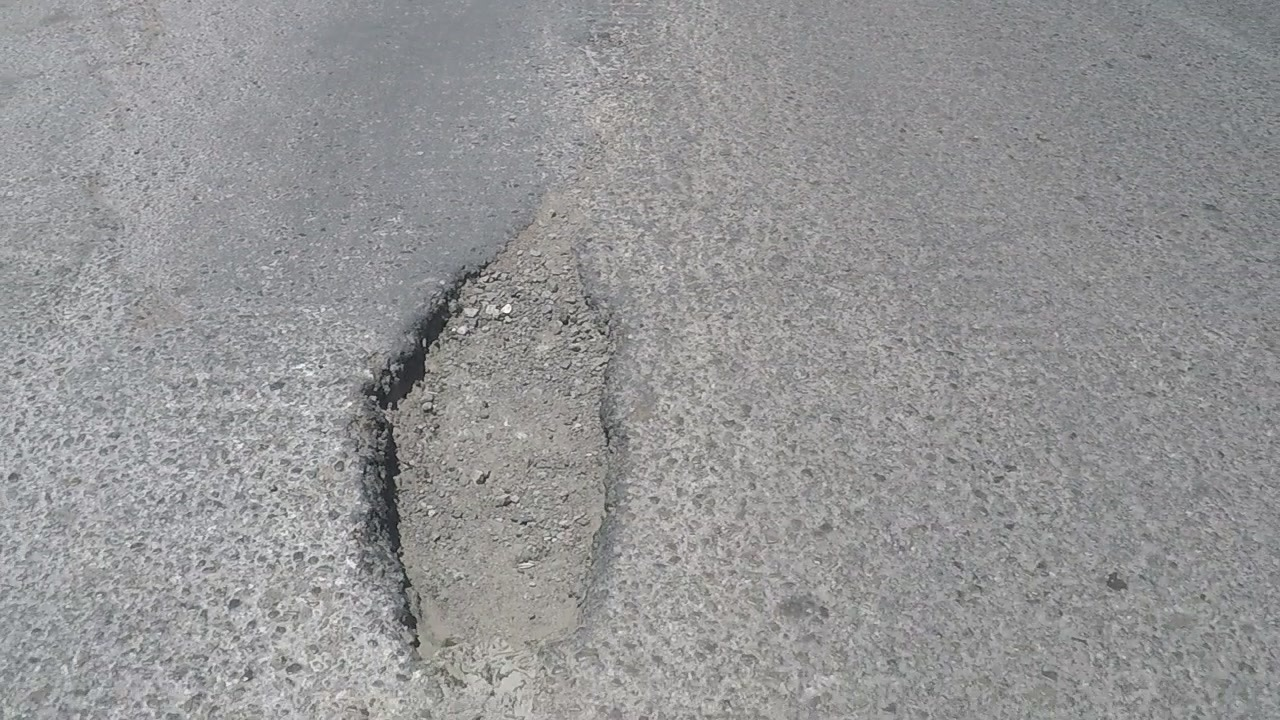
\includegraphics[width=0.4\textwidth]{Images/chapter1/Pothole.jpg}
  \caption{Nids-de-poule}
  \end{figure}
  \newline Un nid-de-poule est une dépression dans la surface d'une route, généralement une chaussée asphaltée, où la circulation 
a enlevé des morceaux cassés de la chaussée. 
C'est généralement le résultat de l'eau dans la structure du sol sous-jacente et du trafic passant sur la zone affectée.
 L'eau affaiblit d'abord le sol sous-jacent; le trafic fatigue et brise la surface asphaltée mal supportée de la zone touchée.
 L'action continue de la circulation éjecte l'asphalte et le sol sous-jacent pour créer un trou dans la chaussée.
\footnote{https://en.wikipedia.org/wiki/Pothole}

\subsection{ Les Ralentisseurs (longues et courtes)}

Normalement fabriquées par l'homme et généralement utilisées pour ralentir les véhicules à proximité des passages pour piétons.
\begin{figure}[h!]
    \center
    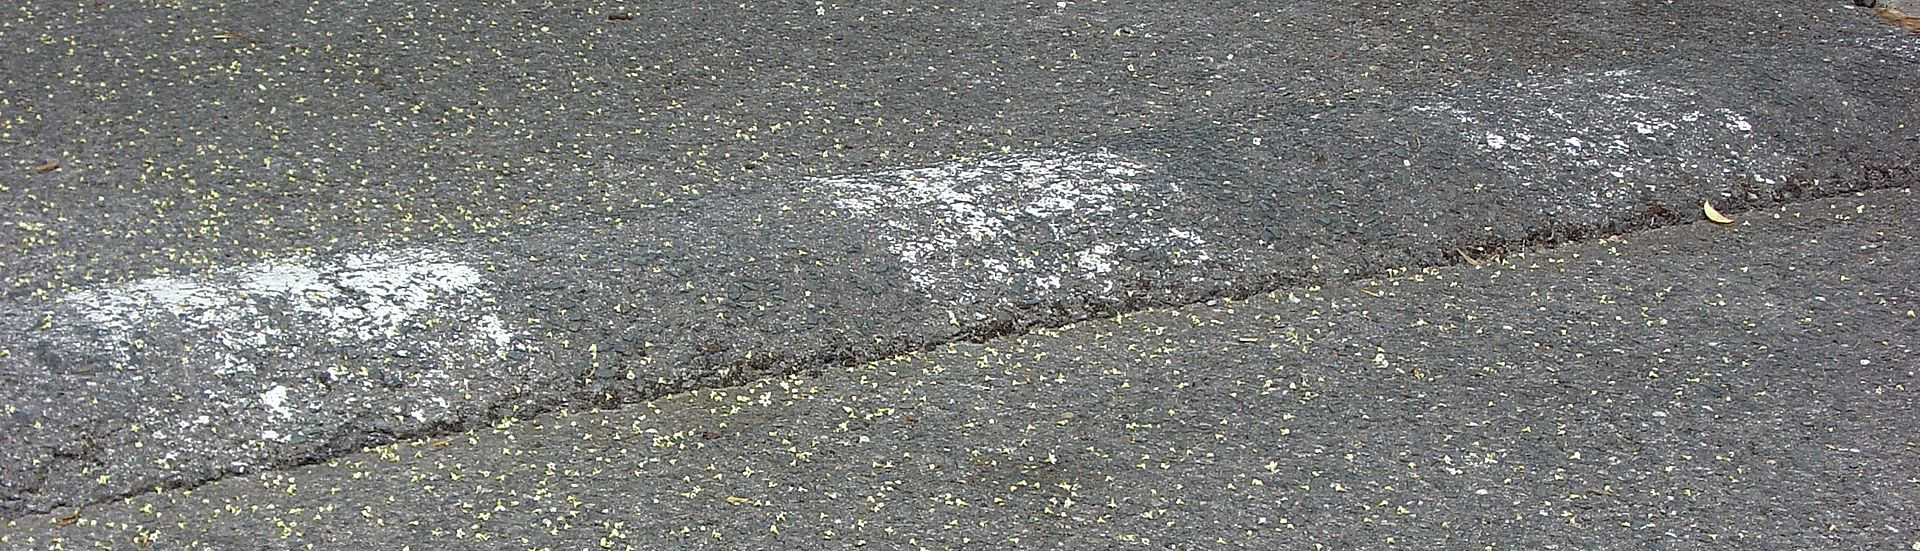
\includegraphics[width=0.9\textwidth]{Images/chapter1/Speedbump.jpg}
    \caption{Ralentisseurs}
    \end{figure}
    On constate le plus souvent qu’ils imposent une limite de vitesse basse, inférieure à 40 km/h ou moins poussant les conducteurs à freiner d’avance.
    Les ralentisseurs en général ne sont pas des anomalies, mais les ralentisseurs mal fait ou ceux qui ont été exposés à des dégâts sans réparation sont considérés comme des anomalies.  
    De plus, leur utilisation est parfois controversée car:
 \begin{itemize}
    \item Ils peuvent augmenter le bruit de la circulation.
    \item Peuvent endommager les véhicules s'ils sont traversés à une vitesse trop élevée et ralentir les véhicules d'urgence.
    \item Les ralentisseurs mal conçus qui se tiennent trop haut ou avec un angle
      trop aigu peuvent perturber les conducteurs et peuvent être difficiles à naviguer pour les véhicules à faible garde au sol,
      même à très basse vitesse.De nombreuses voitures de sport ont ce problème avec de tels ralentisseurs. 
    \item Les ralentisseurs peuvent également présenter de graves dangers pour les motocyclistes et les cyclistes s'ils ne sont pas
    clairement visibles, bien que, dans certains cas, une petite coupure sur le pare-chocs permette à ces véhicules de
     traverser sans obstacle.
  \end{itemize}

  Les ralentisseurs coûtent entre 50 et 200 Dollar et peuvent devoir être remplacés au fil du temps 
   en raison de l'usure 
   \footnote{https://en.wikipedia.org/wiki/Speed\_bump \newline *les ralentisseurs= bosses (i.e bump) *Les nids-de-poule = trou routière (i.e potholes)}. 

\section{Objectifs et analyse des besoins}

Détecter les anomalies d'une route présente un vrai challenge. Avant de commencer le projet,  
 nous sommes amenés à répondre aux questions suivantes :
\begin{itemize}
  \item Quels sont les différents caractéristiques d'une anomalie?
  \item Quels sont les différentes difficultés critères à prendre en compte pour décider si une anomalie est présente?
	\item Peut-on offrir une solution informatique évoluée pour assister à cette décision? Si oui : 
        \begin{itemize}
            \item Comment mesurer Le niveau de qualité de route?
            \item Comment détecter/révéler les différentes causes d'une mauvaise route?
	      	  \item Comment localiser géographiquement chaque détections de ces causes?
	      	  \item Comment présenter cette solution aux usagers de manière simple et efficace ?
	      \end{itemize}
\end{itemize}

   \section{Avantages}
  Développer un outil de route évolué a pour apport :
    \begin{itemize}
	  \item Un gain considérable de temps, efforts humains et une réduction de dépenses.
    \item Une surface de route solide et surtout sans danger pour les piétons et les conducteurs.
    \item Une meilleure circulation en ville en diminuant le nombre d'accidents de route et ainsi réduire les dégâts sur les véhicules.
    \end{itemize}


\section{Approches possibles}  
Pour ce projet, et en raison des conditions routières dans notre zone géographique (Algérie), nous avons décidé de ne nous concentrer que 
sur deux types d'anomalies: les bosses longues et courtes et les nids de poule.\newline
Ainsi une grande vague d'un travail riche et divers a commencé juste pour estimer et étudier les revêtements routiers pour l'améliorer.

\subsection{Une approche utilisant des caméras fixes : }
Cette méthode \cite{kawaiMethodDistinguishRoad2012} distincte  les conditions de surface de la route dans la nuit en utilisant une caméra montée sur une voiture.
En conséquence, elle est basée sur des caractéristiques d'image telles que la "luminance" et la "caractéristique de texture". 
Ils utilisent également les «informations de couleur» afin de prendre en compte l'existence de réverbères et de lampes de signalisation. De cette façon, il a été possible de distinguer les zones routières avec précision, y compris les parties éclairées par les lampadaires et autres sources de lumière en utilisant des informations de couleur. En conséquence, il a été possible d'obtenir une précision de distinction de 96 \% sur sec, 89\% sur mouillé et 96\% sur neige.
L'un des problèmes avec cette méthode le coût des appareils où il est élevé, de plus, les cibles d'estimation sont limitées aux routes qui ont des dispositifs fixes .
\begin{figure}[h!]
    \center
    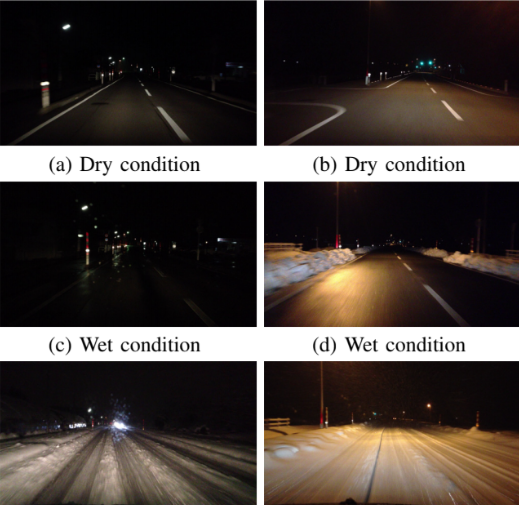
\includegraphics[width=0.45\textwidth]{Images/chapter1/cameraFixe.jpg}
    \caption{Utilisation des cameras fixes}
    \end{figure}
   
\subsection{Une approche utilisant des black-box cameras :}

    Cette approche \cite{joPotholeDetectionSystem2015} propose un nouveau système de détection de nids de poule utilisant une caméra à boîte noire commerciale. Le but de cette recherche est de développer un détecteur de nids-de-poule en utilisant des dispositifs communs qui sont utilisés par de nombreux conducteurs sur une large zone. De plus, les dispositifs devraient fournir une précision de détection élevée à faible coût. L'appareil le plus approprié pour cette exigence est la caméra à boîte noire où ils installent leur algorithme de détection des nids-de-poule, de sorte que tous les véhicules sur les routes seront un détecteur de ces derniers.
    \begin{figure}[h!]
      \center
      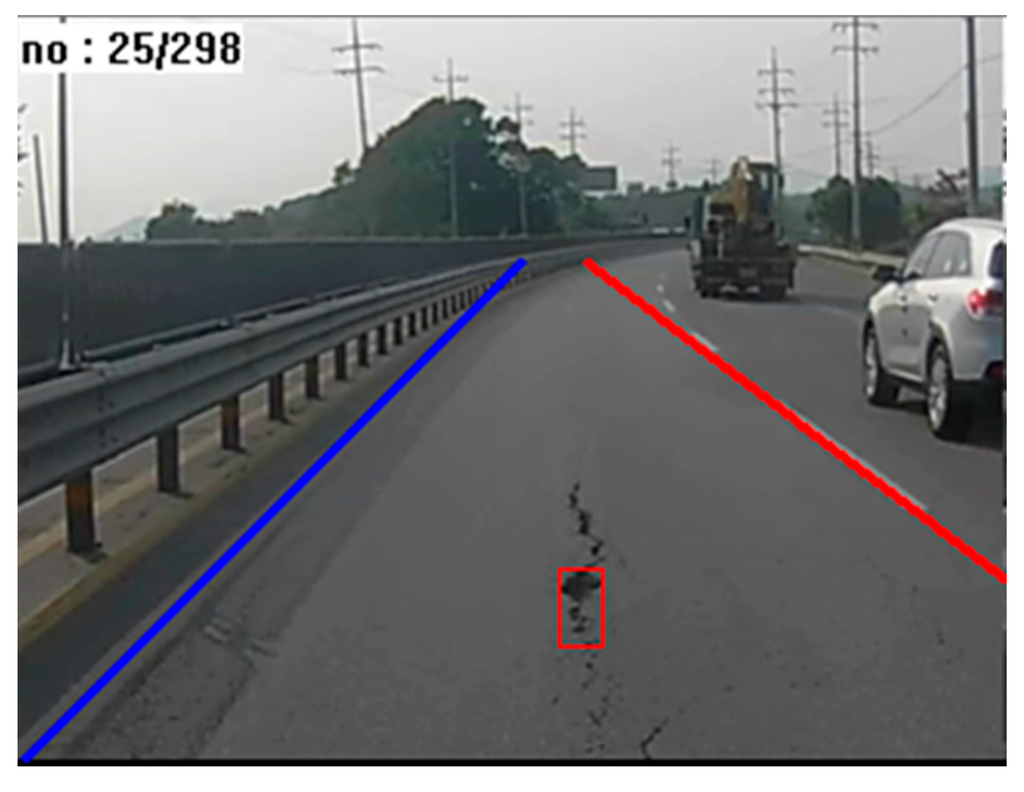
\includegraphics[width=0.51\textwidth]{Images/chapter1/resultatDePotholDetection.jpg}
      \caption{Résultat d'une détection de nid-de-poule}
      \end{figure}

\subsection{Une approche utilisant des capteurs mobiles :}
  Mednis et al\cite{tilluMobileSensorsComponents2019} a conçu un système qui détecte les conditions routières comme les nids-de-poule à l'aide des capteurs intégrés du smartphone. Ils avaient utilisé un capteur accéléromètre du smartphone qui extrait les valeurs et détecte l'existence de nids de poule en temps réel. Ils avaient développé une application sous Android OS et testé en utilisant quatre techniques différentes pour détecter les anomalies routières.
Le système proposé est basé sur une technique de seuil dans laquelle ils ont pu détecter l'état de la surface de la route avec une précision de 90\%.



\section{Solution proposée}
  Nous proposons un outil permettant de :
    \begin{itemize}
      \item Fournir à la direction des travaux public "DTP" un moyen de se renseigner en temps réel sur la qualité des routes afin d'intervenir efficacement et le plus rapidement possible dans les travaux d'entretien.Ceci permettra d’améliorer les manquements cités plus haut.
      \item Mieux assister le conducteur dans sa conduite en prévenant des ralentisseurs/dégradations de la route, afin qu'il adapte sa conduite en fonction.\newline
    \end{itemize}
    Pour cela, nous visons à développer un système qui proposera les fonctionnalités suivantes :
      \begin{itemize}
        \item Détecter les événements (les nids-de-poule et les ralentisseurs dans notre cas) en temps réel.La collecte de données brutes pour un post-traitement hors ligne est classée comme une fonctionnalité supplémentaire. 
        \item Utiliser un smartphone basé sur Android-OS avec des capteurs accéléromètres comme plate-forme matérielle / logicielle. La portabilité vers d'autres plates-formes est classée comme une fonctionnalité supplémentaire.
        \item Pouvoir fonctionner sur différents modèles de smartphones avec différents paramètres. Au cours du processus de mise en œuvre du système, l'ensemble des paramètres minimaux du smartphone doit être déterminé et décrit.
        \item Détecter les événements lors de la conduite dans différents types de véhicules à quatre roues tels que des voitures particulières, des mini-fourgonnettes et des bus. Les véhicules à deux roues tels que les motos et les scooters ne sont pas pris en compte.
      \end{itemize}
      

\renewcommand {\thesection}{\thechapter.\arabic{section}}













